\documentclass[aspectratio=169]{beamer}

\usepackage[utf8]{inputenc} 
\usepackage[T1]{fontenc}
\usepackage[brazil]{babel}
\usepackage{amsmath, amssymb, amsthm, mathtools}
\usepackage{multicol}
\usepackage{multirow}
\usepackage{tikz}
\usepackage{tikz-qtree}
\usepackage{centernot}

\usetikzlibrary{positioning, calc, chains, fit, shapes, automata, trees}

% Tema usado
\usetheme{metropolis}

\title{Pares Ordenados, Produto Cartesiano e Relações.}
\subtitle{CCMP0133 -- Aula 07}
\date{07 de junho de 2022}
\author{Prof. Valdigleis S. Costa\\\url{valdigleis.costa@univasf.edu.br}}
\institute{Universidade Federal do Vale do São Francisco\\Colegiado de Ciência da Computação\\\textit{Campus} Salgueiro-PE}

\newtheorem{defi}{Definição}
\newtheorem{teo}{Teorema}
\newtheorem{col}{Corolário}
\newtheorem{remark}{Observação}

\begin{document}
	\maketitle
	
	\begin{frame}{Roteiro}
		\tableofcontents
	\end{frame}
	
	\section{Pares Ordenados}
	
	\begin{frame}{O objetivo fundamental}
		\begin{defi}[Par ordenado]\label{def:ParOrdenado}
			Sejam $x$ e $y$ elementos em um universo do discurso. O par ordenado entre $x$ e $y$, denotado por $(x, y)$, corresponde a seguinte igualdade.
			\begin{eqnarray*}
				(x, y) = \{\{x\}, \{x, y\}\}
			\end{eqnarray*}
		\end{defi}
		\pause
		Uma questão de interesse:
		\begin{itemize}
			\item Quando dois pares ordenados são igual?
		\end{itemize}
	\end{frame}
	
	\section{Cartesiano}
	
	\begin{frame}{A definição fundamental}
		\begin{defi}[Produto Cartesiano]\label{def:ProdutoCartesiano}
			Sejam $A$ e $B$ dois conjuntos quaisquer. O produto Cartesiano de $A$ e $B$, denotado por $A \times B$, corresponde ao conjunto de todos os pares ordenado onde a primeira componente é um elemento de $A$ e a segunda componente é um elemento de $B$, em notação formal tem-se que:
			\begin{eqnarray*}
				A \times B = \{(x, y) \mid x \in A, y \in B\}
			\end{eqnarray*}
		\end{defi}
		\pause
		Como pode ser usado o conceito de cartesiano na matemática e na computação.
	\end{frame}

	\begin{frame}{Exemplo}
		Dado os seguintes dois conjuntos $\{a, b, c\}$ e $\{-1, 1\}$ tem-se os seguintes produtos Cartesianos:
		\begin{itemize}
			\item[(a)] $\{a, b, c\} \times \{-1, 1\}  = \{(a, 1), (a, -1), (b, -1), (b, 1), (c, -1), (c, 1)\}$.
			\item[(b)] $\{-1, 1\} \times \{a, b, c\}  = \{(1, a), (1, b), (1, c), (-1, a), (-1, c), (-1, b)\}$.
			\item[(c)] $\{a, b, c\} \times \{a, b, c\}   = \{(a, a), (a, b), (a, c), (b, a), (b, b), (b, c), (c, a), (c, b), (c, c)\}$.
			\item[(d)] $\{-1, 1\} \times \{-1, 1\} = \{(1, 1), (1, -1), (-1, 1), (-1, -1)\}$.
		\end{itemize}
	\end{frame}

	\begin{frame}{O quadrado Cartesiano}
		\begin{defi}[Cartesiano quadrado]\label{def:CartesianoQuadrado}
			Seja $A$ um conjunto qualquer. O produto Cartesiano quadrado de $A$, denotado por $A \times A$, corresponde ao produto Cartesiano de A consigo mesmo, em notação formal tem-se que:
			\begin{eqnarray*}
				A \times A = \{(x, y) \mid x, y \in A\}
			\end{eqnarray*}
		\end{defi}
	\end{frame}

	\begin{frame}{Propriedades - (I)}
		\begin{teo}
			Dado dois conjuntos $A$ e $B$ tem-se que, $A \times B = \emptyset$ se, e somente se, $A = \emptyset$ ou $B = \emptyset$.
		\end{teo}
		\begin{teo}
			Dado dois conjuntos $A$ e $B$ tem-se que, $A \times B = B \times A$ se, e somente se, $A = \emptyset$ ou $B = \emptyset$ ou $A = B$.
		\end{teo}
		\begin{teo}
			Dado três conjuntos $A, B$ e $C$ tem-se que, $A \subset B$ se, e somente se, $A \times C \subset B \times C$.
		\end{teo}
		\begin{teo}
			Dado três conjuntos $A, B$ e $C$ tem-se que, $A \subset B$ se, e somente se, $C \times A \subset C \times B$.
		\end{teo}
	\end{frame}

	\begin{frame}{Propriedades - (II)}
		\begin{teo}
			Dado três conjuntos $A, B$ e $C$ tem-se que:
			\begin{itemize}
				\item[(i)] $A \times (B \cap C) = (A \times B) \cap (A \times C)$.
				\item[(ii)] $(A \cap B) \times C = (A \times C) \cap (B \times C)$.
				\item[(iii)] $A \times (B \cup C) = (A \times B) \cup (A \times C)$.
				\item[(iv)] $(A \cup B) \times C = (A \times C) \cup (B \times C)$.
				\item[(v)] $A \times (B - C) = (A \times B) - (A \times C)$.
				\item[(vi)] $(A - B) \times C = (A \times C) - (B \times C)$.
				\item[(vii)] $A \times (B \ominus C) = (A \times B) \ominus (A \times C)$.
				\item[(vii)] $(A \ominus B) \times C = (A \times C) \ominus (B \times C)$.
			\end{itemize}
		\end{teo}
	\end{frame}

	\begin{frame}{Expansão (ou Generalização) dos Pares Ordenados}
		\begin{defi}
			\
			
			Dado $n \geq 2$ e sejam $A_1, A_2, \cdots, A_n$ conjuntos quaisquer, o produto Cartesiano $n$-ário, denotado por $A_1 \times \cdots \times A_n$, corresponde ao conjunto formado por todas as tuplas da forma $(a_1, \cdots, a_n)$ tal que para todo $1 \leq i \leq n$ tem-se que $a_i \in A_i$.
		\end{defi}
		\pause
		\begin{alertblock}{Açúcar Sintático}
			No caso de $A_i = A_j$ para todo $1 \leq i, j \leq n$ e $n \geq$ é comum usar um açúcar sintático\footnote{Açúcar sintático é uma expressão criada em 1964 por Peter J. Landin (1930-2009) em seus trabalhos da década de 60. De forma direta um açúcar sintático diz respeito a uma sintaxe dentro da linguagem formal que tem por finalidade tornar suas construções mais fáceis de serem lidas e expressas, ou seja, um açúcar sintático é uma ferramenta para tornar o uso da linguagem ``mais doce'' (ou amigável) para o uso dos seres humanos.} (\textit{syntactic sugar} em inglês) para representar o produto Cartesiano $n$-ário, em vez de usar, $A_1 \times \cdots \times A_n$ ou mesmo $\displaystyle\prod_{i = 1}^{n} A_i$, em geral é usado a notação $A^n$.
		\end{alertblock}
	\end{frame}

	\begin{frame}{Representação}
		\begin{itemize}
			\item Quando os conjuntos $A_1, A_2, \cdots, A_n$ são todos conjuntos finitos, uma estratégia muito utilizada para se obter e também representar o mecanismo de construção das tuplas $(a_1, a_2, \cdots, a_n)$ pertencentes ao produto Cartesiano $n$-ário $A_1 \times A_2 \times \cdots \times A_n$ é usando a noção de diagrama de árvore.
		\end{itemize}
	\end{frame}

	\begin{frame}{Exemplo De diagrama}
		Dado os conjuntos $\{-1, 1\}, \{a, b\}$ e $\{-1, 1\}$ tem-se que o produto Cartesiano $\{-1, 1\} \times \{a, b\} \times \{-1, 1\}$ pode ser representado pelo diagrama esboçado na Figura \ref{fig:Cartesiano}.

		\begin{figure}[h]
			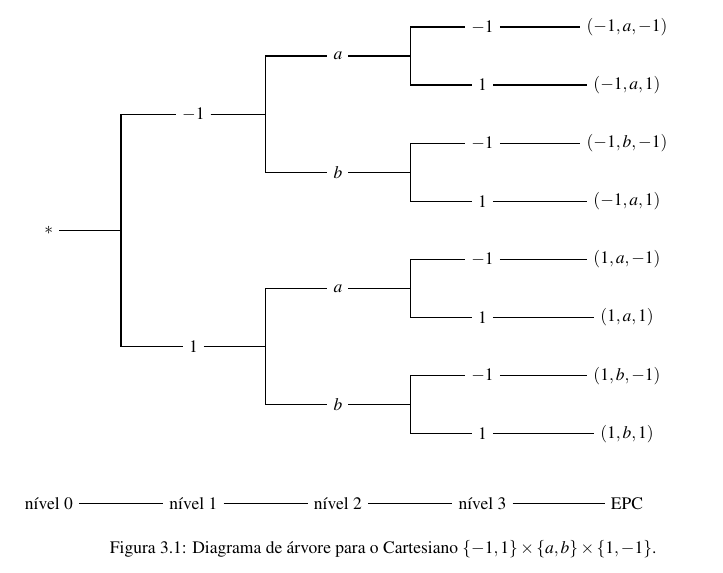
\includegraphics[scale=0.25]{imagem}
			\caption{Diagrama de árvore para o Cartesiano $\{-1, 1\} \times \{a, b\} \times \{1, -1\}$.}
			\label{fig:imagem}
		\end{figure}
	\end{frame}

	\section{Relações}

	\begin{frame}{As Relações Básicas}
		\begin{defi}[Relação binária]\label{def:RelacaoBinaria}
			Seja $A$ e $B$ dois conjuntos, uma relação $R$ de $A$ em $B$ é qualquer subconjunto de $A \times B$, isto é, $R \subseteq (A \times B)$.
		\end{defi}
		\pause
		\begin{alertblock}{Açúcar Sintático}
			Dado $R$ uma relação binária de $A$ em $B$ a sintaxe da teoria dos conjuntos e de pares ordenados permite que seja escrito que $(x, y) \in R$, entretanto, está escrita é geralmente substituída por $x\mathrel{R}y$. E no caso de $(x,y) \notin R$ é escrito simplesmente $x\centernot{R}y$.
		\end{alertblock}
	\end{frame}

	\begin{frame}{Componentes Básicos}
		\begin{defi}[Domínio e Imagem]\label{def:DominioImagemRelacoes}
			Seja $R$ uma relação de $A$ em $B$, o domínio de $R$, denotado por $Dom(R)$, corresponde ao conjunto de todos os elementos de $A$ que são a primeira coordenada de $x\mathrel{R}y$, ou seja, 
			$$Dom(R) = \{x \in A \mid x\mathrel{R}y\}$$
			e a imagem de $R$, denotada por $Ima(R)$, corresponde ao conjunto de todos os elementos de $B$ que são a segunda coordenada de $x\mathrel{R}y$, ou seja, 
			$$Ima(R) = \{y \in B \mid x\mathrel{R}y\}$$
		\end{defi}
	\end{frame}

	\begin{frame}{Dual Relacional}
		\begin{defi}[Relação inversa]\label{def:RelacaoInversa}
			Seja $R$ uma relação. A relação inversa (ou oposta) de $R$, denotada por $R^{-1}$, corresponde ao seguinte conjunto:
			$$R^{-1} = \{(y,x) \mid x\mathrel{R}y\}$$
		\end{defi}
	\end{frame}

	\begin{frame}{Operação Básica e Propriedades}
		\begin{defi}[Composição de relações]\label{def:ComposicaoRelacoes}
			Seja $R_1$ uma relação de $A$ em $B$ e seja $R_2$ uma relação de $B$ em $C$, a composição de $R_1$ e $R_2$, denotada por $R_1 \bullet R_2$, corresponde ao seguinte conjunto:
			$$R_1 \bullet R_2 = \{(x, z) \mid (\exists y \in B)[x\mathrel{R_1}y \text{ e } y\mathrel{R_2}z] \}$$ 
		\end{defi}
		\pause
		\begin{teo}
			Seja $R_1$ uma relação de $A$ em $B$ e seja $R_2$ uma relação de $B$ em $C$, então tem-se que:
			\begin{itemize}
				\item[(i)] $Dom(R_1 \bullet R_2) \subseteq Dom(R_1)$.
				\item[(ii)] $Ima(R_1 \bullet R_2) \subseteq Ima(R_2)$.
			\end{itemize}
		\end{teo}
	\end{frame}
	
	\begin{frame}{Mais Propriedades}
		\begin{teo}
			Seja $R_1$ e $R_2$ relações de $A$ em $B$. Se $R_1 \subseteq R_2$, então para toda relação $R_3$ de $B$ em $C$ tem-se que $(R_1 \bullet R_3) \subseteq (R_2 \bullet R_3)$.
		\end{teo}
		\begin{col}
			Se $R_1, R_2, S_1, S_2$ são relações tais que $R_1 \subseteq R_2$ e $S_1 \subseteq S_2$ com $Ima(R_1) = Dom(S_1)$ e $Ima(R_2) = Dom(S_2)$, então $(R_1 \bullet S_1) \subseteq (R_2 \bullet S_2)$.
		\end{col}
		\begin{teo}
			Seja $R_1$ uma relação de $A$ em $B$ e seja $R_2$ uma relação de $B$ em $C$ tem-se que $(R_1 \bullet R_2)^{-1} = R_2^{-1} \bullet R_1^{-1}$.
		\end{teo}
		\begin{teo}
			Seja $R_1$ uma relação de $A$ em $B$ e seja $R_2$ uma relação de $B$ em $C$ e $R_3$ uma relação de $C$ em $D$ tem-se que $(R_1 \bullet R_2) \bullet R_3 = R_1 \bullet (R_2 \bullet R_3)$.
		\end{teo}
	\end{frame}
\end{document}
